\chapter{Análisis de algoritmos}\label{cap:Analisis}

\section{Introducción}
Para el estudio de las técnicas basadas en proximidad, vamos a usar como
fuente principal de estudio el libro de Charu C. Aggarwal
\cite{aggarwalOutlierAnalysis2017}.

En primer lugar, vamos a analizar los conceptos básicos de las técnicas basadas
en proximidad. Estas técnicas definen un punto de datos como un valor 
atípico cuando su localidad (o proximidad) está poblada escasamente.
Existen varias formas de definir la proximidad de un punto de datos.
Estas definiciones son sutilmente diferentes entre sí, pero son lo suficientemente
similares como para agruparlas y realizar un tratamiento unificado 
dentro de un solo tipo. Las formas más comunes de definir la proximidad 
para la detección de anomalías son las siguientes:


\begin{itemize}
    \item \textbf{Basado en cluster.} La no pertenencia de un punto de 
    datos a cualquiera de los grupos, su distancia a otros grupos,
    el tamaño del grupo más cercano o una combinación de estos factores
    se utilizan para cuantificar la puntuación final de la anomalía.
    El problema de clustering tiene una relación complementaria
    con el problema de detección de valores atípicos, en el que los 
    puntos pertenecen a grupos o deben considerarse valores atípicos.
    \item \textbf{Basados en distancias.} La distancia de un punto de 
    datos a su k-vecino más cercano (u otra variante) se utiliza para 
    definir la proximidad. Los puntos de datos con grandes distancias 
    a sus k-vecinos más cercanos, se definen como valores atípicos. 
    Los algoritmos basados en la distancia generalmente realizan el 
    análisis con una granularidad mucho más detallada que los otros dos 
    métodos. Por otro lado, esta mayor granularidad a menudo tiene un 
    costo computacional significativo.
    \item \textbf{Basados en densidad.} La cantidad de otros puntos 
    dentro de una región local específica (una cuadrícula o 
    región basada en la distancia) de un punto de datos, 
    se utiliza para definir la densidad local. Estos valores de 
    densidad local se pueden convertir en la puntuación final. 
    También se pueden usar otros métodos basados en kernel o métodos 
    estadísticos para la estimación de la densidad. La principal diferencia 
    entre el clustering y los métodos basados en la densidad es que los 
    métodos de agrupación en clústeres dividen los puntos de datos, 
    mientras que los métodos basados en la densidad dividen el espacio 
    de datos.

\end{itemize}

No podemos negar que todas estas técnicas están estrechamente 
relacionadas porque se basan en alguna noción de proximidad (o similitud).
La principal diferencia está en el nivel de detalle con el cual se 
estima la proximidad. Es obvio que cada forma diferente de definir la 
proximidad y, por tanto, que es una anomalía, conlleva ciertas ventajas
y desventajas. En muchos casos, es difícil diferenciar en cuál de las
definiciones estamos trabajando ya que es muy usual usar más de un concepto
a la vez. Es por ello que también queda justificado su agrupación para un análisis conjunto.

Como ya hemos anunciado antes, una diferencia importante entre los 
métodos basados en distancias y los otros dos tipos, radica en el
nivel de granularidad en el que se realiza el análisis. Tanto en los 
métodos basados en clustering, como en densidad, los datos quedan 
agrupados antes del análisis y el cálculo de puntuación de anomalía.
Esta agrupación se realiza ya sea mediante la partición de los puntos
o del espacio. Cada punto del conjunto de datos se compara con las 
distribuciones en estos datos pre-agrupados para el análisis. Por
otro lado, en los métodos basados en distancias, la distancia del
k-vecino más cercano a los puntos de datos originales (o una variante 
similar) se calcula como la puntuación de anomalía. Por lo tanto, el 
análisis en los métodos del vecino más cercano se realiza a un nivel de 
granularidad más detallada que los métodos de agrupamiento. Dicho de otra manera
se analizan todos los puntos. Esta mayor granularidad conlleva una desventaja,
estos métodos proporcionan diferentes compensaciones entre la eficacia y la 
eficiencia para conjuntos de datos de diferentes tamaños. Los métodos en los
que calculamos el vecino más cercano pueden tener una complejidad $O(N^{2})$ para
calcular todas las distancias del vecino k más cercano para un conjunto de
datos de tamaño N. Es fácil de ver de dónde surge dicha
complejidad, ya que para cada punto deberemos de calcular la distancia con
el resto de puntos. Esta complejidad se puede reducir o acelerar si 
usamos alguna técnica de indexación o poda.

Pero el uso de estas técnicas no será algo trivial que nos solucione todos
nuestros problemas, las técnicas de indexación y poda generalmente 
funcionan bien solo en algunas configuraciones restringidas, como los 
conjuntos de datos de baja dimensionalidad. Además, la poda no está diseñada
para el problema que nos ocupa ya que puede ser altamente interesante tener
la puntuación final de todos los puntos, aunque no se considere anomalía. Por
ellos la poda solo podrá usarse en aquellas configuraciones en las que la
respuesta sea una etiqueta binaria que indica si un punto es anomalía.
al contrario de lo que esto nos podría hacer pensar, las técnicas 
del k-vecino más cercano o más conocidas como k-nn, son técnicas
con una alta popularidad y su uso es muy frecuente para diversas aplicaciones.
Esto se debe a que tales métodos a menudo son capaces de proporcionar un
análisis más detallado y preciso. Este hecho se amplifica en conjuntos de 
datos pequeños donde el agrupamiento o el análisis de densidad no es posible
o los resultados que ofrece son complicados. En definitiva, la elección de 
un modelo, definición o técnica, depende de la naturaleza de los datos y
su tamaño.

Las técnicas basadas en la proximidad de los datos, están diseñadas naturalmente
para detectar tanto el ruido como las anomalías. A pesar de ello existen 
métodos que se adecuan más para cada tarea. Por ejemplo, la definición
de una baja pertenencia de un punto a un grupo de datos, está diseñada
naturalmente para la detección de ruido. Mientras que, por otro lado 
una alta desviación o escasez de densidad o altas distancias pueden 
detectar mejor las anomalías. A pesar de ello los métodos basados en la 
pertenencia tienen también popularidad ya que son muy intuitivos y 
se dispone de una fácil explicación a la puntuación de una anomalía.
De hecho, varios métodos se basan en este tipo de definiciones, ya que 
por su simplicidad, se pueden generalizar fácilmente a casi todos los 
tipos de datos, tanto datos de series temporales, como datos de secuencia
o datos de gráficos.

Ahora vamos a analizar y explicar más detalladamente cada uno de los subgrupos
que hemos expuesto. Como ya hemos comentado anteriormente, aunque exista
un concepto principal en algunos algoritmos, la realidad es que muchos 
pueden interpretarse desde varias perspectivas y es difícil su clasificación
en un tipo u otro. A pesar de ello todas siguen siendo técnicas basadas 
en proximidad.


\section{Métodos basados en clustering}
Como ya comentamos anteriormente existe una fuerte conexión entre la detección
de anomalías y el clustering. Si vemos el problema de la detección de anomalías
desde este nuevo enfoque y con una visión simplista, podemos determinar que cada
punto puede ser miembro de un clúster o ser una anomalía. Aquellos puntos que
no se agrupen dentro de un clúster se pueden definir entonces como anomalía.
En el clustering, el objetivo principal es dividir los puntos en subconjuntos
densos. Por otro lado, en la detección de anomalías el objetivo es identificar
los puntos que no encajan fácilmente o de forma natural en estos subconjuntos
densos. De hecho, los algoritmos de clustering reportan valores atípicos como 
un producto secundario de su análisis.

Parece que hemos encontrado una solución fácil y buena a nuestro problema,
pero, sin embargo, es importante entender que usar solo la relación
complementaria de la pertenencia a los grupos para definir los
valores atípicos da como resultado el descubrimiento no solo anomalías si no
también del ruido. Esto se debe a que la no pertenencia de un punto a ningún
grupo de datos es una razón bastante directa para medir el nivel de
desviación de un punto de datos de los patrones normales.  Por ejemplo, 
normalmente un conjunto de puntos no suele estar muy concentrado en un único
punto, por tanto, un punto de datos que se encuentra en la periferia
de un grupo grande es muy diferente de uno que está completamente 
aislado de todos los otros grupos. Además, todos los puntos de datos
en grupos muy pequeños a veces también pueden considerarse anomalías. 
En definitiva, cuando se utiliza la agrupación en clústeres para la 
detección de anomalías, se utiliza un enfoque más matizado (que el de 
la no pertenencia a un grupo) para calcular las puntuaciones de los 
valores atípicos.


Podemos definir una definición simple para realizar una puntuación de anomalías
utilizando las distancias de los puntos de los puntos de datos a los centroides
generados al agrupar en clúster. Específicamente, la distancia de un punto
al centroide del grupo más cercano se puede usar como una buena característica
para la puntuación de valor atípico de un punto de datos. Dado que los grupos
pueden tener diferentes formas y orientaciones, una excelente medida de la
distancia que se debe utilizar es la distancia de \textit{Mahalanobis}, que escala los
valores de distancia según las variaciones locales del grupo, a lo largo de las
direcciones de la correlación. 

Vamos a ver cómo podemos aplicar la distancia \textit{Mahalanobis}. En primer
lugar, consideramos un conjunto de datos que contiene $k$ clústeres. Supongamos
que el grupo $rth$ en el espacio de $d$ dimensiones tiene un vector fila $d$-dimensiones
denotado por $\overline{\mu_r}$ que contiene la media de cada atributo. Por
otro lado disponemos de una matriz de covarianzas de dimensiones $d$ x $d$
definida como $\Sigma_r$. La entrada $(i,j)$ de esta matriz nos proporciona
la covarianza local entre las dimensiones $i$ y $j$ en el clúster. Con esto podemos
definir el cuadrado de la distancia \textit{Mahalanobis} entre un punto 
definido como vector-fila $\overline{X}$ con la siguiente expresión:

\begin{center}
    $MB(\overline{X}, \overline{\mu_r}, \Sigma_r)^2 = (\overline{X} - \overline{\mu_r})
    \Sigma_r^{-1} (\overline{X} - \overline{\mu_r})^T$
\end{center}
Después de que los puntos de datos se hayan calificado con la distancia
local de Mahalanobis, cualquier método se puede aplicar
como detector de anomalías para convertir estas puntuaciones en etiquetas binarias.

El efecto de la distancia de Mahalanobis es proporcionar
una normalización estadística basada en las características de un punto
de datos particular. Incluso aunque las distancias pequeñas a lo largo de las 
direcciones en las que se producen las variaciones del grupo son pequeñas
pueden ser estadísticamente significativas dentro de esa localidad de datos.
De manera análoga, las grandes distancias a lo largo de las direcciones
en las variaciones del grupo que son grandes pueden no ser,
estadísticamente significativas dentro de esa localidad de datos.
Dicho enfoque producirá resultados más refinados que un uso global
de la distancia Euclidia, porque se adapta mejor a la localidad de
datos en cuestión.

Para remarcar las propiedades y ventajas que nos ofrece el uso de la distancia
Mahalanobis vamos a plantear el ejemplo planteado en \cite{aggarwalOutlierAnalysis2017}:
\begin{figure}[h]
    \center{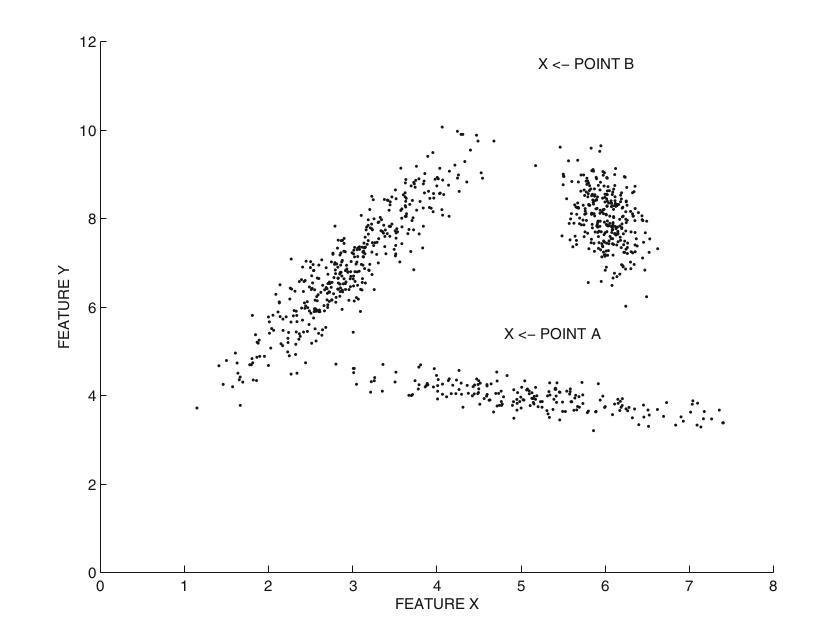
\includegraphics[width=\textwidth]
    {imagenes/distancia_mahalanobis.jpeg}}
    \caption{\label{fig:distance_maha} Ejemplo uso de la distancia Mahalanobis}
\end{figure}

Como podemos ver, en este ejemplo el punto A debería ser considerado una
anomalía con mayor facilidad que el punto B. Esto se debe a que el punto 
A no sigue ningún patrón y es algo claramente fuera de lo normal. Sin embargo
el punto B a pesar de estar alejado del clúster, puede verse como un punto
perteneciente al clúster ya que sigue el patrón, aunque se aleje más. Si aplicamos
la distancia Euclidia, el punto B está más lejos de los centroides que el
punto A. Por lo que el punto B obtendría una puntuación mayor que A. Sin 
embargo, si usamos la distancia Mahalanobis solventamos estos inconvenientes.


Además de los criterios basados en la distancia, es común usar el número
de puntos pertenecientes al conjunto como un componente de la puntuación
de valor atípico. Por ejemplo, el logaritmo negativo de la fracción de
puntos en el grupo más cercano se puede utilizar como un componente de
la puntuación de anomalía. Podemos crear dos vectores de puntuaciones
de N-dimensiones basados en los criterios de distancia y cardinalidad,
normalizar cada uno y luego agregarlos.

También debemos mencionar que los métodos basados en clustering tienen una alta
variabilidad de predicción ya que estos dependen de la elección del modelo especifico,
la inicialización aleatoria o la configuración de parámetros. Todos estos 
factores influyen en los resultados finales. Para ello será aconsejable realizar
varias mediciones y usar la media.

Como conclusión final de este tipo de métodos vamos a mencionar las ventajas
y desventajas que estos ofrecen. Una de las principales ventajas es que existen
algoritmos de clustering relativamente rápidos y que no alcanzan la complejidad
cuadrática de los algoritmos basados en distancias, como veíamos anteriormente.
La principal desventaja de los métodos de clustering es que no siempre proporcionan
la información al nivel de detalle requerido. La granularidad de los métodos de análisis
de valores atípicos es generalmente mejor cuando se utilizan cálculos de
distancia directamente con los puntos de datos originales, en lugar de con
respecto a representantes agregados, como los centroides de los clústeres.



\section{Métodos basados en distancias}
Los métodos basados en distancias son una clase popular de algoritmos 
de detección de anomalías en una amplia variedad de tipos de datos.
Estos definen puntuaciones de los valores atípicos en función de las 
distancias del vecino más cercano. El ejemplo más simple es el caso en 
el que la distancia del vecino más cercano $k$ de un punto se
usa como su puntuación. Como podemos ver es un método simple y por ello,
a menudo es fácil generalizar esta técnica a otros tipos de datos como 
datos categóricos, datos de texto, datos de series de tiempo y datos de 
secuencia.

Los métodos basados en la distancia funcionan con la suposición natural 
de que las distancias del vecino $k$ más cercano de las anomalías
son mucho mayores que las de los puntos de datos normales.


Como ya hemos mencionado con anterioridad, las técnicas basadas en distancias
nos proporcionan una gran granularidad de análisis en comparación con los métodos
de clustering. Esta propiedad puede permitir una capacidad más refinada 
para distinguir entre ruido y anomalías. Para analizar este hecho vamos a
recordar el ejemplo de la Introducción donde como veíamos no era fácil
distinguir entre ruido y anomalías.

\begin{figure}[h]
    \center{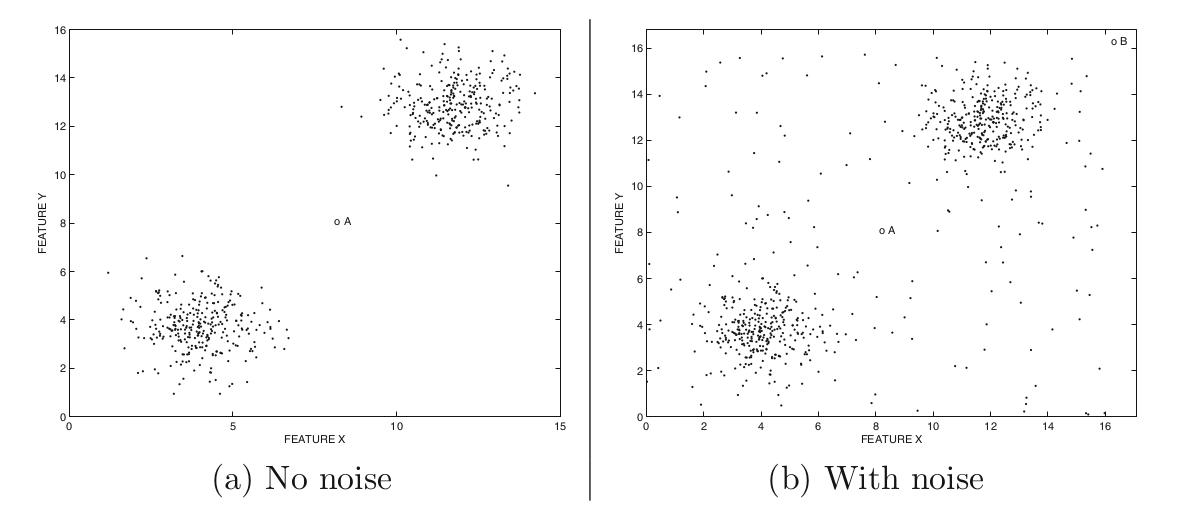
\includegraphics[width=\textwidth]
    {imagenes/ejemplo_basico.jpeg}}
    \caption{\label{fig:my-label} Ejemplo de datos con ruido}
\end{figure}

Como podemos ver en la figura, un algoritmo de clustering no sería capaz de 
distinguir entre ruido y anomalías. Esto se debe a que la distancia al centroide 
de clúster más cercano para el punto de datos $A$ seguirá siendo la misma en 
ambos casos. Por otro lado, un algoritmo vecino más cercano k (k-nn) distinguirá entre 
estas situaciones porque los puntos de datos ruidosos se incluirán entre 
las evaluaciones de distancia. Por otro lado, el enfoque de clustering no 
podrá distinguir estas situaciones con un resultado tan bueno porque los 
centroides de cada clúster son relativamente insensibles al ruido en 
los datos. Por supuesto, también es posible modificar métodos basados en
clústeres para incluir los efectos del ruido. En esos casos, los dos
enfoques convergen y pasan a ser enfoque muy similares. Esto se debe a 
que como hemos mencionado anteriormente, aunque los consideremos tipos distintos,
en realidad los dos tipos de métodos están estrechamente relacionados.
 

La funcionalidad de este tipo de métodos es muy alta, también pueden 
identificar grupos aislados de anomalías estrechamente relacionados.
Por ejemplo, para identificar un grupo pequeño que contiene $k_0$
puntos de datos, es necesario usar un valor de $k \geq k_0$ en el algoritmo
de vecino más cercano. Aunque dichas anomalías también se pueden identificar
mediante métodos de clustering al establecer un umbral en la cantidad de
puntos en cada clúster, a veces estos puntos pueden agruparse en clúster 
y sesgar los centroides correspondientes. Esto como podemos imaginar puede 
afectar el proceso de puntuación atípica de manera muy negativa.


El resultado más general de los métodos basados en la distancia es en 
forma de score. Si necesitamos la puntuación de todos los puntos será
necesario el cálculo de las distancias relativas a cada punto y, por tanto,
necesitamos una complejidad de $O(N^{2})$. En el caso de que necesitemos una
respuesta binaria, si se identifica un punto como anomalía es posible la 
aplicación de varios tipos de poda y estructuras de indexación, con lo que
conseguiremos una alta ganancia de velocidad.


\subsection{Métodos basados en distancias para puntuación}
La puntuación de anomalía basada en la distancia de un punto
se fundamenta en la distancia del vecino más cercano $k$ . 
Hay dos variaciones simples de este mecanismo de puntuación conocidos como
el k-nearest neighbor exacto y el k-nearest neighbor promedio:




\begin{itemize}
    \item \textbf{k-nn exacto.} Se usa como puntuación la distancia al
    $k$ vecino más lejano donde $k$ es un parámetro que debemos establecer.
    Debemos tener en cuenta que no podemos usar la distancia del punto
    así mismo ya que esto podría afectar a los resultados. El problema
    de este enfoque es la elección correcta del valor para $k$. Un buen
    resultado dependerá de nuestra elección. En problemas no supervisados,
    como la detección de valores atípicos, a menudo no hay manera de 
    ajustar los parámetros con métodos como la validación cruzada,
    ya que tales métodos requieren un conocimiento extra de la información.
    \item \textbf{k-nn con media.} En este caso se realiza el cálculo del
    $k$ vecino más cercano. En este caso en lugar de usar solo la distancia
    de este vecino se usa el promedio de los $k$ vecinos más cercanos, es decir,
    aquellos que su distancia es menor a la del $k$ vecino.
    de datos. En este caso el parámetro $k$ no influye tan fuerte como en el caso
    anterior. Por tanto si conocemos el valor correcto de $k$, el k-nn exacto
    nos proporciona mejores resultados, pero si no podemos mitigar este error
    usando el promedio de las distancias.
    \item \textbf{k-nn con media armónica.} Igual que en el caso anterior
    solo que usamos la media armónica para calcular la puntuación. Debemos
    tener cuidado de eliminar los valores repetidos. Este tipo de media siempre
    este dominada por distancias pequeñas y por tanto si usamos un valor alto
    para k, incluso en el caso de usar $ k = N$, conseguiremos una alta robustez.
    
\end{itemize}

\subsection{Métodos basados en distancias para etiquetas binarias}
En esta variedad de los métodos basados en distancias se obtiene una salida
de etiqueta binaria, que determina si un punto es una anomalía o no. Este
enfoque limita el número de aplicaciones en el cual podemos hacer uso de 
esta técnica, pero tiene una gran ventaja. En el caso anterior hablábamos de 
que era totalmente necesario una complejidad de $O(N^2)$, en este caso con
el uso de etiquetas binarias podemos aplicar ciertas técnicas de poda.


En este esquema solo los scores más altos serán considerados como anomalías 
y no debemos preocuparnos por la puntuación específica de cada punto.
para conseguir este objetivo, la técnica que principalmente se usa, es determinar
un umbral de puntuación $\beta$ a partir del cual, los puntos que lo superen se consideran
anomalías. También podemos verlo como establecer un umbral de la distancia mínima para 
ser considerado anomalía.


Ambos enfoques son en esencia idénticos y debemos de remarcar que conllevan 
añadir un nuevo parámetro $\beta$ que se usará para determinar el umbral. 
Este hecho aumenta la complejidad de nuestro problema y es que es necesario
una correcta elección de dicho parámetro y será fundamental en los resultados.


Por tanto, el proceso se compondrá de un cálculo de todas las distancias y una
posterior clasificación para aplicar el umbral. Esto como podemos imaginar sigue
siendo un cálculo bastante costoso. Para obtener una mejora será necesario
realizar una poda. 


Existen varías técnicas como la poda basada en celdas donde se divide el espacio
en celdas. Para no entrar en detalles la idea básica será evitar el cálculo
repetitivo de otros puntos en la misma celda ya que los resultados serán muy similares.
Este algoritmo comienza a complicarse ya que ahora además se debe de ajustar 
el tamaño de dichas celdas.


Existen más técnicas de poda, con procedimientos más complejos como puede ser la 
poda basada en índices o la poda basada en muestreo. Todas estas técnicas son
interesantes, aunque en nuestro caso no son relevantes ya que nos centramos en técnicas
que aportan como resultado la puntuación final de anomalía.


\subsection{Ventajas y desventajas}
Los métodos basados en la distancia tienen una serie de ventajas 
sobre las técnicas basadas en clustering, debido a la granularidad 
más detallada del análisis. Por ejemplo, los algoritmos basados en la 
distancia pueden distinguir entre ruido y anomalías mucho mejor que los 
basados en técnicas de clustering. Además, los métodos basados en la
distancia también pueden encontrar grupos aislados de valores atípicos
al igual que los métodos de clustering. Sin embargo, los métodos de 
clustering tienen la ventaja de que
pueden proporcionar información sobre las distribuciones locales 
de puntos para definir distancias. También existen casos como el que veíamos
en la figura \ref{fig:distance_maha}, donde la estructura del clúster local se
puede utilizar para definir una distancia de Mahalanobis localmente 
sensible, que es mucho más efectiva en este caso, que una aplicación ciega de
la distancia Euclidia. También es posible la combinación y realización de
un enfoque basado en distancias que use la distancia Mahalanabis.

Aunque los métodos basados en la densidad que se explican más adelante
incorporan algunos conceptos de localidad, no pueden proporcionar el 
nivel detallado de información local que una combinación efectiva de 
un enfoque basado en clustering y distancia puede proporcionar. En esta
tendencia existen multitud de investigaciones, las cuales buscan agrupar
las ventajas que proporcionan cada tipo de algoritmos. Por un lado, la eficiencia
que aportan los métodos basados en clustering y por otro lado la granularidad
y los buenos resultados que ofrecen los métodos basados en distancias.

 




\section{Métodos basados en densidad}

Los métodos basados en la densidad utilizan la cantidad de puntos 
en regiones específicas del espacio para definir valores atípicos. 
Están muy estrechamente relacionados con el clustering y los métodos 
basados en la distancia. En realidad, algunos de estos algoritmos 
pueden considerarse más fácilmente como clustering o basados en la 
distancia, según cómo se presenten. Esto es porque la idea de distancias,
clustering y la densidad están estrechamente relacionadas y son dependientes
entre sí. Esta relación la veremos más clara cuando expliquemos los algoritmos
implementados, ya que, aunque la mayoría se pueden considerar de densidad, pueden
considerarse también basados en distancias o clustering, simplemente viendo 
los métodos desde otro enfoque.


Para comprender mejor el enfoque basado en densidad y la capacidad de detección
de estos métodos basados en localidad, vamos a ver un ejemplo que se muestra en
la siguiente figura del libro \cite{aggarwalOutlierAnalysis2017}:

\begin{figure}[h]
    \center{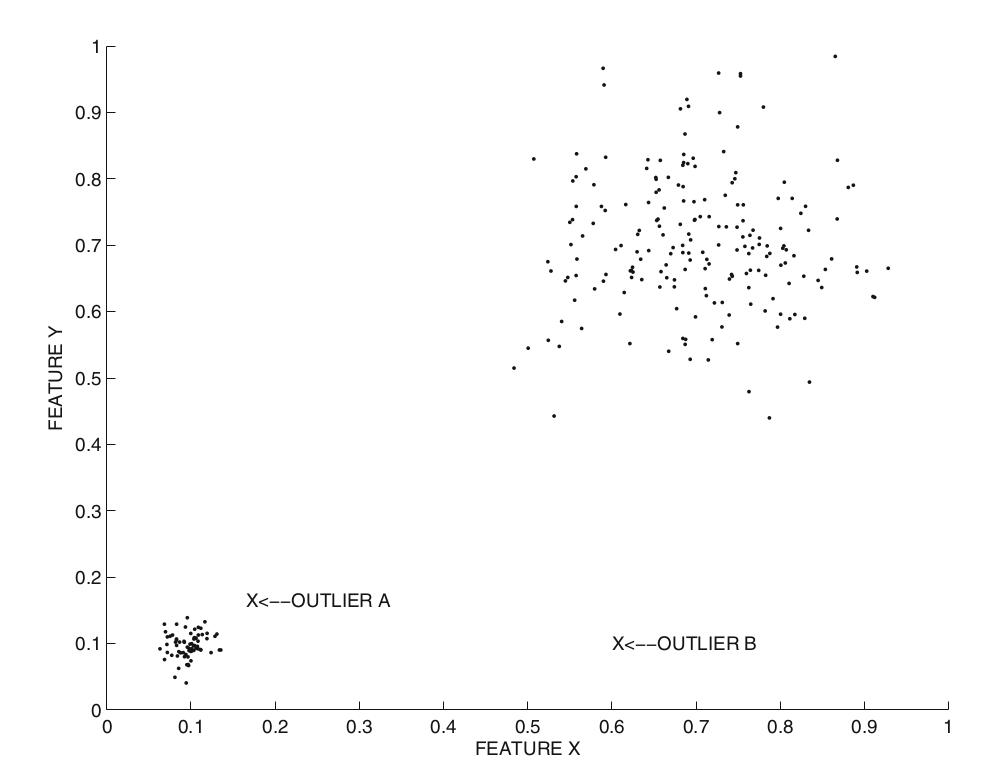
\includegraphics[width=\textwidth]
    {imagenes/ejemplo-densidad.jpeg}}
    \caption{\label{fig:densidad} Ejemplo detección por densidad}
\end{figure}

Esta figura contiene dos anomalías etiquetadas con A y B.Además, la figura 
contiene dos grupos, uno de los cuales es mucho más disperso que el otro.
Es evidente que los algoritmos basados en la distancia no pueden descubrir la
anomalía A, a menos que el algoritmo utilice un umbral de distancia muy pequeño.
El uso de este umbral para la distancia tan pequeño conlleva que muchos puntos
del grupo disperso también sean considerados anomalías, llevando a un resultado 
totalmente erróneo. Esto también significa que la clasificación devuelta por un
algoritmo basado en la distancia es incorrecta cuando hay heterogeneidad 
significativa en las distribuciones locales de los datos. Sin embargo, que mide la 
densidad de cada punto, podemos determinar que A y B son anomalías sin necesidad 
de asignar una alta puntuación al grupo de puntos disperso ya que estos detectarán
una mayor densidad a su alrededor. Por ello estos algoritmos son muy interesantes.


Gran parte del trabajo en clustering basado en densidad generalmente 
se ha centrado en cuestiones de densidad de datos variable en lugar de la forma 
y orientación variable de los grupos, como comentábamos en el análisis de la figura
\ref{fig:distance_maha}


Otros métodos combinan los algoritmos de \textbf{k-nn} con variaciones locales de 
densidad. El más claro ejemplo de aplicación de estos conceptos es \textbf{LOF} 
\cite{breunigLOFIdentifyingDensitybased2000}, algoritmo que explicaremos más adelante
y que hemos implementado en nuestra biblioteca.